\label{chap_post_process}

This chapter describes the post-process of the field-data output from {\psiboil}.
The field-data file is: 
    \begin{itemize}
	\item written in Tecplot ASCII data format,
	\item with the file extension {\tt "dat"},
	\item including the grid data (always) and variables (optional).
    \end{itemize}
Here all the variables in the file are defined at cell centers. It is worth reminding that the {\tt Vector} variable, e.g. velocity vectors and body-force vectors, is defined at the cell faces in {\tt PSI-BOIL}, the so-called staggered grid variable arrangement. However, the velocity vectors are defined at the cell centers in the Tecplot file. This means that the velocity at cell center is the average of those at the face centers. The {\tt Scalar} variables computed in {\tt PSI-BOIL} are directly output to the file and they can be visualized by a post-process software without averaging process.

\section{Data format}
\label{sec_data_format}
There are two types of data formats for Tecplot data: ASCII and binary. The file size of ASCII is about three times larger than the binary file. Thus, it is better to keep the field-data as the binary format rather than the ASCII to save the disk space.

\section{Serial computation}

The field-data file contains the entire computational domain. {\tt preplot} converts an ASCII file to the binary format. First we compile the executable file {\tt preplot} as follows.
\begin{verbatim}
	> cd Src/Utilities/Gather 
	> g++ preplot.cpp -DPLOT3D -DUNIXX -DLINUX -o preplot
	> cp preplot ~/bin/.
\end{verbatim}
Here we assume that {\tt \~/bin} is the directory, to which a path is set. 

We use Section~\ref{sec_domains} ({\tt 05-04-main.cpp}) as an exercise. The field data output from {\tt PSI-BOIL} is {\tt dom.dat}. To change the file format of {\tt dom.dat} from ASCII to binary:
\begin{verbatim}
	> preplot dom.dat
\end{verbatim}
The output of this operation is {\tt dom.plt}. Following visualization software can open the field-data file. 
\begin{itemize}
	\item Tecplot: Tecplot can open both the ASCII and binary file. 
	\item VisIt: VisIt can import only the binary file. The ASCII file output from {\tt PSI-BOIL} cannot be imported by VisIt because of its bug: VisIt does not recognize the comment line in the file starting with {\tt \#}.
	\item Paraview: it can import only the ASCII file.
\end{itemize}

If there are multiple {\tt *.dat} files, it is cumbersome to perform {\tt preplot} for each file. The script file {\tt dopreplot}  perform {\tt preplot} for all the files in the current directory.
\begin{verbatim}
	> cp ./Utilities/Gather/dopreplot ~/bin/.
	> dopreplot 
\end{verbatim}

\section{Parallel computation}
If a simulation is performed in the parallel computation, the computational domain is decomposed into the sub-domains, the total number of sub-domain corresponds to that of processes used for the computation. We compute the case Section~\ref{sec_domains} ({\tt 05-04-main.cpp}) using eight processes:
\begin{verbatim}
	> mpiexec -np 8 ./Boil 
\end{verbatim}
The output files are {\tt dom\_p000.dat}, {\tt dom\_p001.dat},..., and {\tt dom\_p007.dat}. Figure ~\ref{fig_tec_8domains} shows the grid lines of the eight domains. The thick blue lines indicates the edges of the domains.  

\begin{figure}[ht]
	\centering
	\setlength{\unitlength}{1mm}
	\begin{picture}( 100, 80)(0,0)
		\thickbox{ 100}{ 80}
		\put(0,0){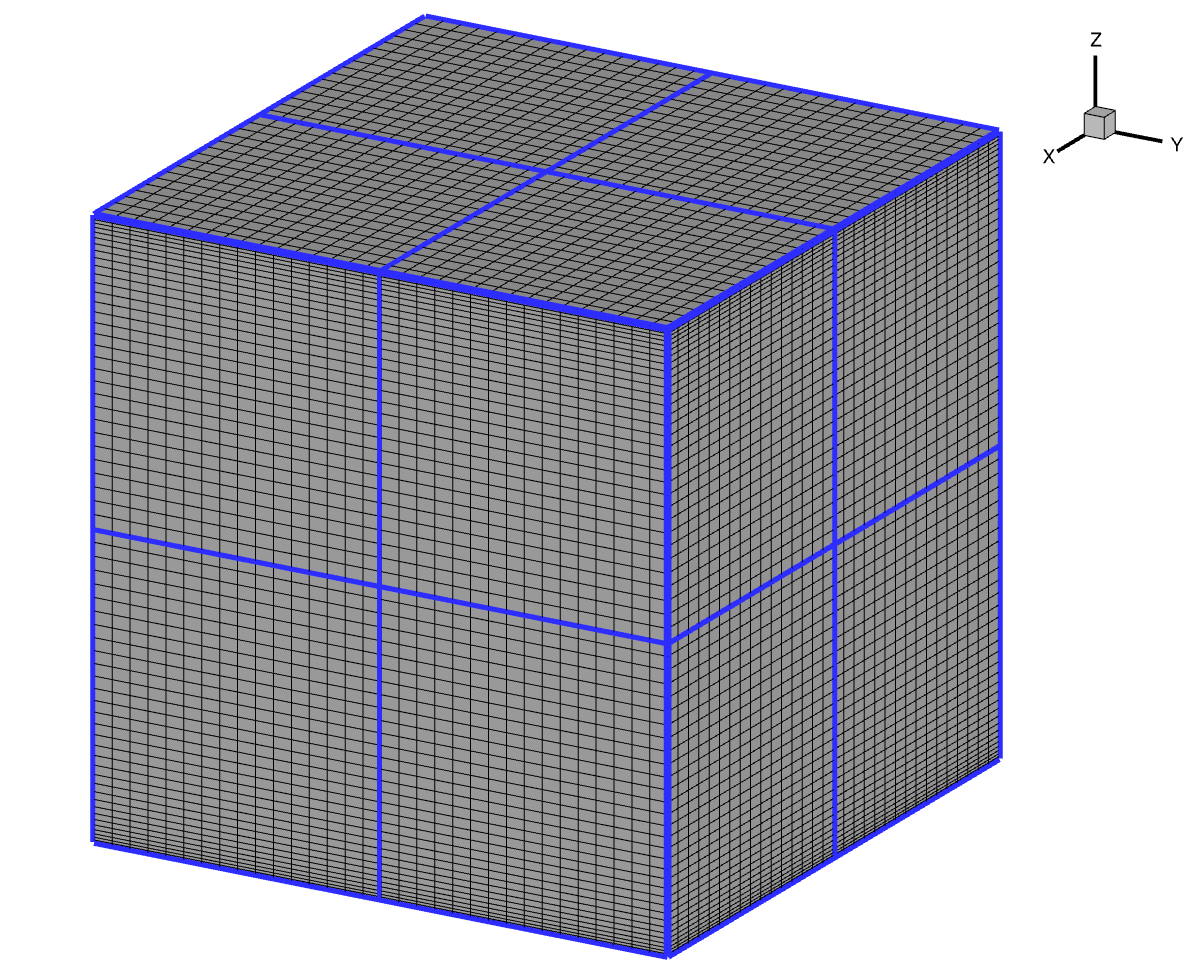
\includegraphics[scale=0.2]{Figures/10-01-8domains.png}}
	\end{picture}
	\caption{Visualization of domain decomposed grid.} 
	\label{fig_tec_8domains}
\end{figure}

Handling of the eight domains, i.e. decomposed domains, is not straightforward, and it is better to combine all the domains into one. For this purpose, we use {\tt gather.exe}. To compile {\tt gather.exe},
\begin{verbatim}
	> cd Src/Utilities/Gather 
	> gfortran -cpp -DVISIT gather.f90 ./tecio64.a -lm -lstdc++ -fcray-pointer -o gather.exe
\end{verbatim}
If you use Intel compiler instead of {\tt gfortran},
\begin{verbatim}
	> ifort -fpp -DVISIT gather.f90 ./tecio64.a -lm -lstdc++ -o gather.exe
\end{verbatim} 
Then copy {\tt gather.exe} and {\tt dogather} to {\tt \~/bin/.}.

\begin{verbatim}
	> cp gather.exe dogather ~/bin/.
\end{verbatim} 

Here {\tt dogather} is the script, which automatically perform {\tt gather.exe}, in the same way as {\tt dopreplot}. First, we use {\tt gather.exe}:
\begin{verbatim}
	> gather.exe
	 Input number of processor
	8
	Input number of digit for time step
	6
	Input start of time step
	-1
	Input end of time step
	-1
	Input time step increment
	1
	Input common file name.
	Example: uvw-c-press_p
	dom_p
	nstart=          -1
	dom_p000.dat
	dom_p001.dat
	...
	dom_p007.dat
	fname_out=dom_pall.plt
	1 X
	2 Y
	3 Z
	WITH BUFFER=  F
	icmax,jcmax,kcmax=          32          32          64
	Output to dom_pall.plt
\end{verbatim} 
Here {\tt Input number of processor} is 8 because 8 processes are used (mpiexec -np 8). Since the input file names, e.g. dom\_p000.dat, do not include time step information, we enter arbitrary natural number as {\tt Input number of digit for time step}, and -1 as {\tt Input start of time}, implicitly indicating that the time step is not included in the file name. The output file is {\tt dom\_pall.plt}, which is written in the binary format. The input files, {\tt dom\_p00*.dat}, are automatically removed by {\tt gather.exe}. Note that Tecplot and VisIt can open the binary format file, but Paraview cannot.

To automatically perform {\tt gather.exe} for all the {\tt *dat} files exists in the directly without manual input of the parameters, we may execute:
\begin{verbatim}
	> dogather
\end{verbatim} 
 
\section{VisIt}
\label{sec_visit}
Here are some useful tips for using VisIt. Please refer to the manual for a complete description (https://visit-dav.github.io/visit-website/).

\subsection{Contour map (Visit:Pseudocolor)}
You may need to visualize a distribution of {\tt Scalar} variable, e.g. pressure or temperature. In visit, the distribution of scalar is called {\tt Pseudocolor}. To draw it, click "Add" in Plots, and select {\tt Pseudocolor}. To display the distribution on a sliced plane:\\
{\tt Right click on Pseudocolor > Operators > Slicing > Slice}
We can specify the slicing surface on the popup window, but we need to uncheck the checkbox of {\tt Project to 2D} as shown in Figure~\ref{fig_visit_slice}.

\begin{figure}[ht]
	\centering
	\setlength{\unitlength}{1mm}
	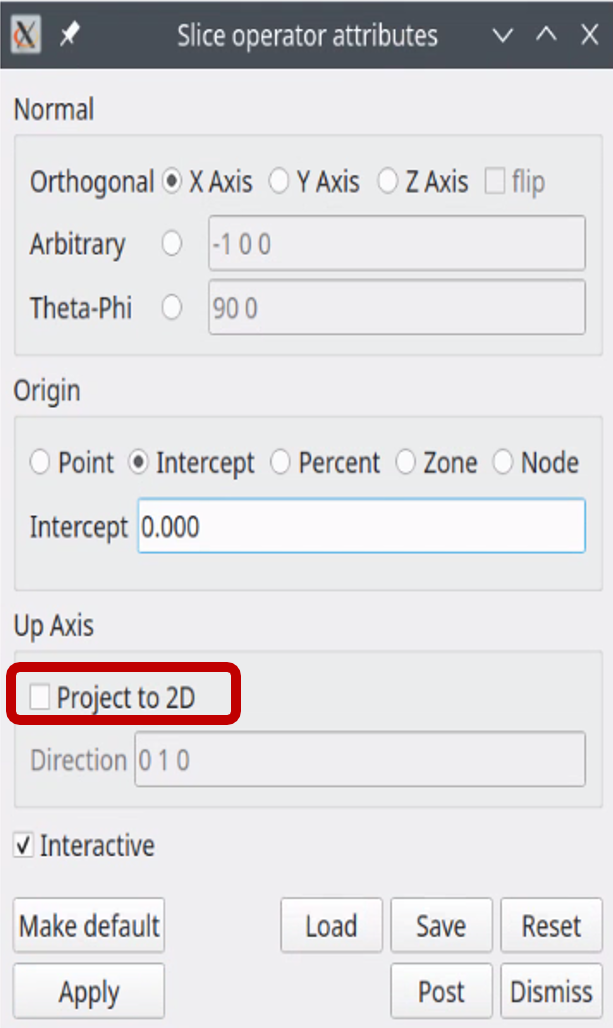
\includegraphics[height=8cm]{Figures/10-01-visit-slice.png}
	\caption{Definition of slicing surface.} 
	\label{fig_visit_slice}
\end{figure}

\subsection{Isosurface (Visit:Contour)}
An isosurface is called {\tt Contour} in VisIt. An isosurface is required for example to draw a liquid-vapor interface, which is the isosurface at 0.5 of the color function. Click "Add" in Plots, and select {\tt Contour}.


\subsection{Velocity vector}
To draw velocity vectors, we need to define {\tt Vector mesh variable} as follows. \\
{\tt Menu > Controls > Expressions}\\
On the Popup window of Expressions, first click {\tt "New"} and then enter the parameters as shown in Figure~\ref{fig_visit_vector}.

\begin{figure}[ht]
	\centering
	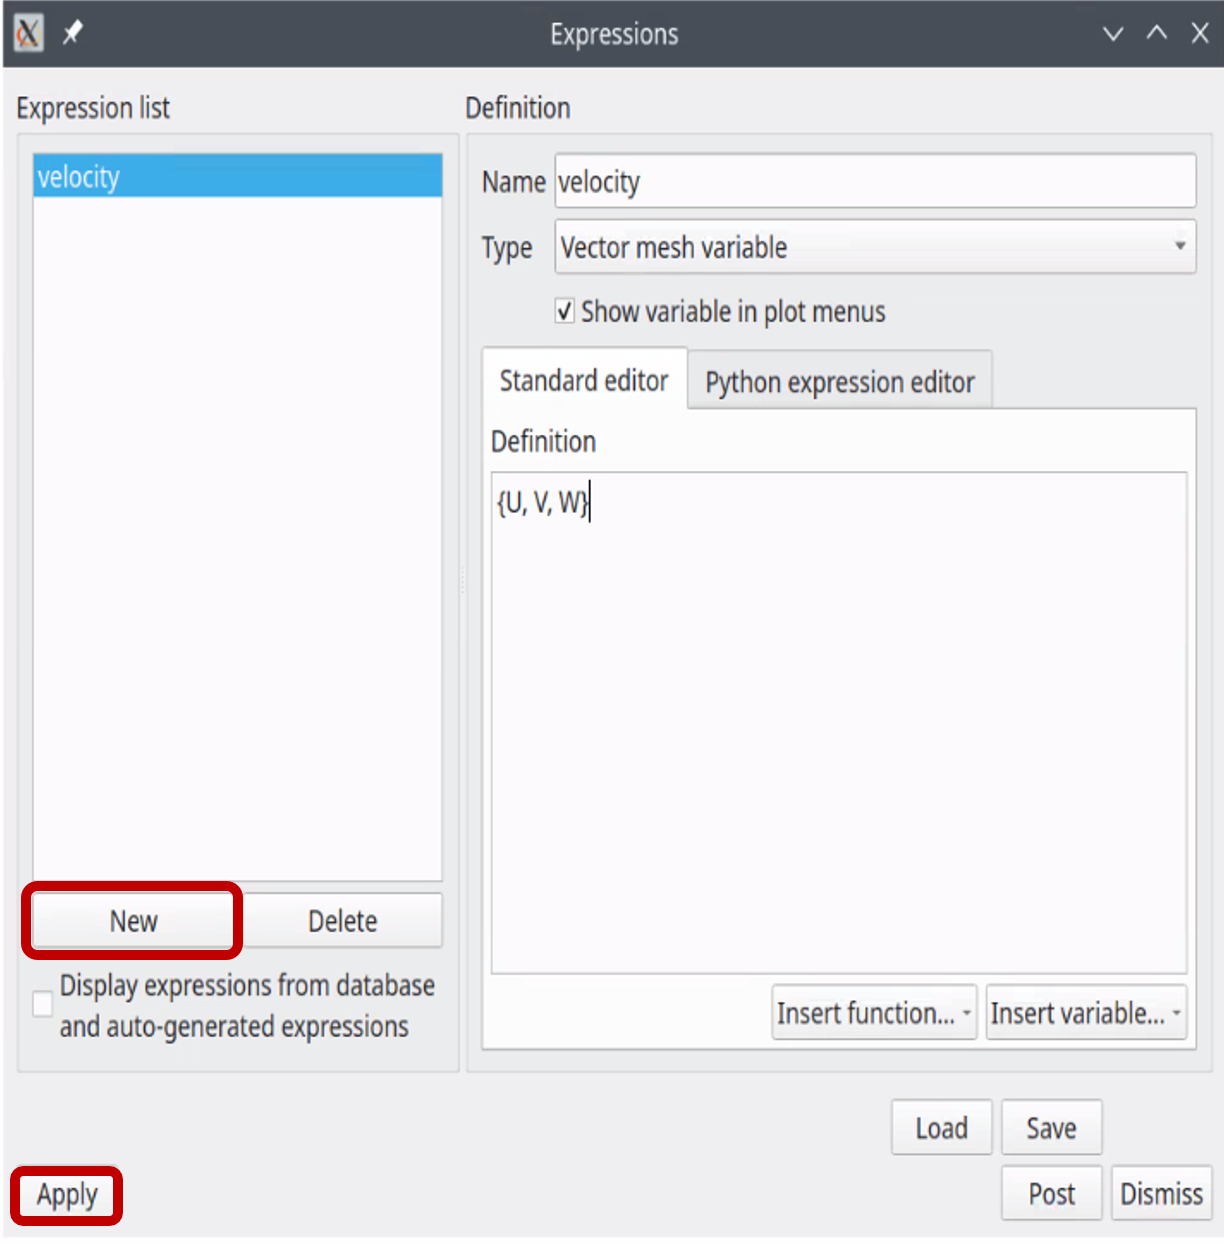
\includegraphics[height=8cm]{Figures/10-01-visit-vector.png}
	\caption{Definition of velocity vector.} 
	\label{fig_visit_vector}
\end{figure}

\subsection{Integral of variable}
To calculate volume integral of a variable,\\
{\tt Menu > Controls > Query}.
